\section{Testing Strategy}\label{sec:testing}

\subsection{Approach}
Testing was done in four layers. \emph{Component tests} exercised \texttt{Course}, \texttt{AssessmentComponent} and \texttt{IndividualMarksManager} from a console demonstration program. \emph{Integration tests} combined the domain classes with \texttt{Database} and the role classes. \emph{System tests} drove the Swing interface by hand with normal, boundary and invalid input. \emph{Regression checks} were repeated after each refactor (the \texttt{Module} to \texttt{Course} rename, the normalisation fix and the move from the console to the GUI). Expected results were worked out by hand before running each case, using the default weights of 30, 30 and 40.

\subsection{Test cases}
\begin{table}[htbp]
\centering
\small
\renewcommand{\arraystretch}{1.1}
\caption{Selected test cases with inputs and expected results.}
\label{tab:tests}
\begin{tabularx}{\textwidth}{@{}l >{\raggedright\arraybackslash}p{3.7cm} >{\raggedright\arraybackslash}p{3.3cm} X@{}}
\toprule
\textbf{ID} & \textbf{Scenario} & \textbf{Input} & \textbf{Expected result}\\
\midrule
T1 & Complete record & 60, 70, 80 & Final mark $18+21+32 = 71.0$; statistics calculated.\\
T2 & Update a mark & Exam 80 changed to 90 & Final mark recalculated to $75.0$.\\
T3 & Missing mark & Exam left blank & Row flagged, final mark withheld, status names the exam.\\
T4 & Boundary marks & 0 and 100 & Accepted and calculated correctly.\\
T5 & Out-of-range mark & 105 or $-5$ & \texttt{IllegalArgumentException}; error dialog; nothing saved.\\
T6 & Non-numeric mark & \texttt{abc} & Error dialog; record unchanged.\\
T7 & Blank or duplicate course code & Empty field, existing code & Rejected with a message; no file created.\\
T8 & No row selected & Press Update & Warning asking for a selection.\\
T9 & Unknown student number & Search for an absent ID & Message that no record was found.\\
T10 & Import with missing header & File without a required column & Rejected with a readable error; table unchanged.\\
T11 & Name containing a comma & \texttt{Surname, Name} & Saved quoted and loaded back as one field.\\
T12 & Export without extension & Name \texttt{results} & File written as \texttt{results.csv}.\\
\bottomrule
\end{tabularx}
\end{table}

All cases behaved as listed. The full run, including the interface cases, is shown in the demonstration recording submitted with this report.

\subsection{Evidence}
Figure~\ref{fig:evidence} shows console evidence for the component tests T1 to T3.

\begin{figure}[htbp]
\centering
\begin{subfigure}[t]{0.29\textwidth}\centering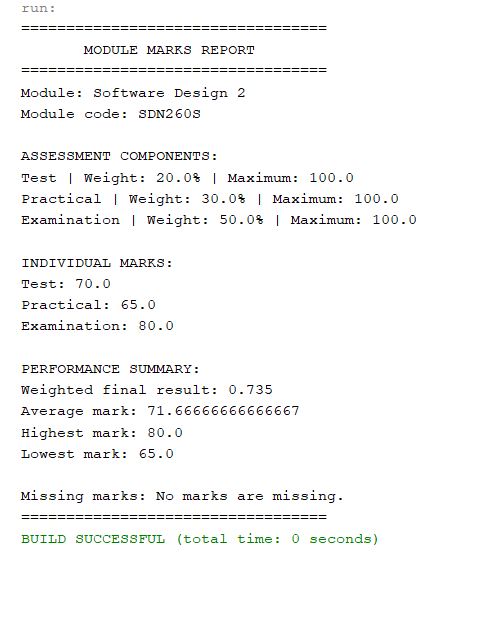
\includegraphics[height=4.3cm]{Images/ch4_complete_marks_test.png}\caption{T1: complete.}\end{subfigure}\hfill
\begin{subfigure}[t]{0.29\textwidth}\centering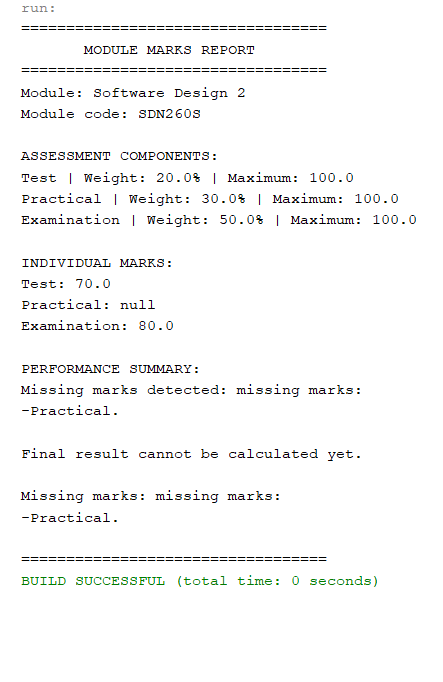
\includegraphics[height=4.3cm]{Images/ch4_missing_mark_test.png}\caption{T3: missing.}\end{subfigure}\hfill
\begin{subfigure}[t]{0.29\textwidth}\centering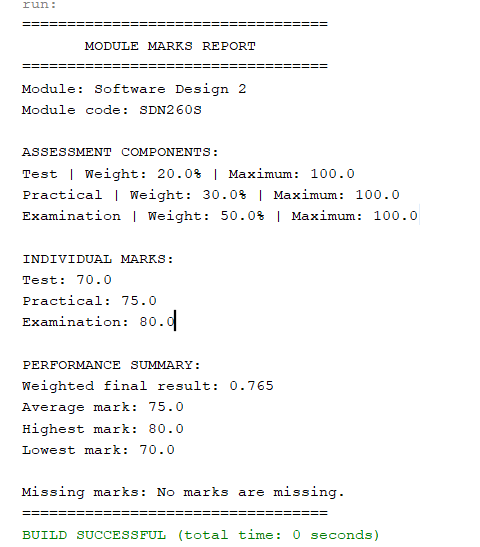
\includegraphics[height=4.3cm]{Images/ch4_updated_mark_test.png}\caption{T2: updated.}\end{subfigure}
\caption{Console output for the component tests.}
\label{fig:evidence}
\end{figure}

\subsection{Defects found}
Testing and review exposed four issues. (1) The demonstration program crashed when it asked for a result on an incomplete record, because it did not check \texttt{hasMissingMarks()} before calling the calculation; the check was added. (2) Final marks were wrong when assessments had different maximum marks, which led to the normalisation fix. (3) Inconsistent test CSV files caused null pointer errors on import, so validation and clear error prompts were added before records are read. (4) Review of \texttt{saveData} showed that it replaces the whole file, so data would be lost if a course were saved before it was loaded; course data is therefore loaded when a course is selected. A check before overwriting an exported file is still open (Section~\ref{sec:concl}).
